%%%%%%%%%%%%%%%%%%%%%%%%%%%%%%%%%%%%%%%%%%%%%%%%%%%%%%%%%%%%%%%%%%%%%%%%%%%%%%%%%%%%%%%%%%%%%%%%%%%%%%%%%%%%%%%%%%%%%%%%%%%%%%%%%%%%%%%%%%%%%%%%%%%%%%%%%%%
% This is just an example/guide for you to refer to when submitting manuscripts to Frontiers, it is not mandatory to use Frontiers .cls files nor frontiers.tex  %
% This will only generate the Manuscript, the final article will be typeset by Frontiers after acceptance.   
%                                              %
%                                                                                                                                                         %
% When submitting your files, remember to upload this *tex file, the pdf generated with it, the *bib file (if bibliography is not within the *tex) and all the figures.
%%%%%%%%%%%%%%%%%%%%%%%%%%%%%%%%%%%%%%%%%%%%%%%%%%%%%%%%%%%%%%%%%%%%%%%%%%%%%%%%%%%%%%%%%%%%%%%%%%%%%%%%%%%%%%%%%%%%%%%%%%%%%%%%%%%%%%%%%%%%%%%%%%%%%%%%%%%

%%% Version 3.4 Generated 2018/06/15 %%%
%%% You will need to have the following packages installed: datetime, fmtcount, etoolbox, fcprefix, which are normally inlcuded in WinEdt. %%%
%%% In http://www.ctan.org/ you can find the packages and how to install them, if necessary. %%%
%%%  NB logo1.jpg is required in the path in order to correctly compile front page header %%%

\documentclass[utf8]{frontiersSCNS} % for Science, Engineering and Humanities and Social Sciences articles
%\documentclass[utf8]{frontiersHLTH} % for Health articles
%\documentclass[utf8]{frontiersFPHY} % for Physics and Applied Mathematics and Statistics articles

%\setcitestyle{square} % for Physics and Applied Mathematics and Statistics articles
\usepackage{url,hyperref,lineno,microtype,subcaption}
\usepackage[onehalfspacing]{setspace}
\usepackage{adjustbox}
\usepackage{graphicx}

\linenumbers


% Leave a blank line between paragraphs instead of using \\


\def\keyFont{\fontsize{8}{11}\helveticabold }
\def\firstAuthorLast{Sample {et~al.}} %use et al only if is more than 1 author
\def\Authors{First Author\,$^{1,*}$, Co-Author\,$^{2}$ and Co-Author\,$^{1,2}$}
% Affiliations should be keyed to the author's name with superscript numbers and be listed as follows: Laboratory, Institute, Department, Organization, City, State abbreviation (USA, Canada, Australia), and Country (without detailed address information such as city zip codes or street names).
% If one of the authors has a change of address, list the new address below the correspondence details using a superscript symbol and use the same symbol to indicate the author in the author list.
\def\Address{$^{1}$Laboratory X, Institute X, Department X, Organization X, City X , State XX (only USA, Canada and Australia), Country X \\
$^{2}$Laboratory X, Institute X, Department X, Organization X, City X , State XX (only USA, Canada and Australia), Country X  }
% The Corresponding Author should be marked with an asterisk
% Provide the exact contact address (this time including street name and city zip code) and email of the corresponding author
\def\corrAuthor{Corresponding Author}

\def\corrEmail{email@uni.edu}

\begin{document}
\onecolumn
\firstpage{1}

\title[Running Title]{Article Title} 

\author[\firstAuthorLast ]{\Authors} %This field will be automatically populated
\address{} %This field will be automatically populated
\correspondance{} %This field will be automatically populated

\extraAuth{}% If there are more than 1 corresponding author, comment this line and uncomment the next one.
%\extraAuth{corresponding Author2 \\ Laboratory X2, Institute X2, Department X2, Organization X2, Street X2, City X2 , State XX2 (only USA, Canada and Australia), Zip Code2, X2 Country X2, email2@uni2.edu}


\maketitle
\begin{abstract}

\section{}
% For full guidelines regarding your manuscript please refer to \href{http://www.frontiersin.org/about/AuthorGuidelines}{Author Guidelines}.
% As a primary goal, the abstract should render the general significance and conceptual advance of the work clearly accessible to a broad readership. References should not be cited in the abstract. Leave the Abstract empty if your article does not require one, please see \href{http://www.frontiersin.org/about/AuthorGuidelines#SummaryTable}{Summary Table} for details according to article type. 

\tiny
 \keyFont{ \section{Keywords:} keyword, keyword, keyword, keyword, keyword, keyword, keyword, keyword} %All article types: you may provide up to 8 keywords; at least 5 are mandatory.
\end{abstract}

\section{INTRODUCTION}

% For Original Research Articles \citep{conference}, Clinical Trial Articles \citep{article}, and Technology Reports \citep{patent}, the introduction should be succinct, with no subheadings \citep{book}. For Case Reports the Introduction should include symptoms at presentation \citep{chapter}, physical exams and lab results \citep{dataset}.
meta-analysis, IVGTT and minimal model, SI and then SG as a potential therapeutic target, Physiologic of SG, population approach, previous papers,
pooled study, algorithm

\section{MATERIALS AND METHODS}

\subsection{Clinical study data}
In this study, we pooled the glucose-insulin concentration-time data of 497 subjects from 51 groups, with a total of 8024 measurements . In Table. \ref{tab:studies}, we summarize the pooled studies by each study group, with the cohorts, original sex information, mean demographic characteristics, study types and references displayed. The whole dataset includes 228 healthy subjects, 115 obese subjects and 154 type 2 diabetes patients (T2DM). Obese subjects were classified as people in good general health with a body mass index (BMI) larger than 28 $kg/m^2$. Patients in the T2DM cohort had type 2 diabetes at the baseline or had a placebo administration. 229 of the subjects underwent an insulin-modified IVGTT and 268 had an IVGTT. For the subjects with missing continuous covariates, mean values reported in the original papers were used (Table. \ref{tab:studies}). For 40 subjects from study groups 31, 32, 33, 34, the values of height, weight and BMI were missing, and only the ranges of BMI were reported. We used a virtual population generator (PopGen, \cite{McNally2015}) to generate virtual subjects for these four groups and applied the calculated mean weight to those subjects. Then, the heights were imputed using the equation: $H=\sqrt{weight/BMI}$ and the given mean BMI value. The sex information of 18 subjects from two study groups 6 and 36 was missing but the sex ratio (i.e., male/female) was mentioned in the literature, so random assignment was used to fill in the sex value. For 41 subjects from groups 9, 10, 28, 29, 40, no sex information about gender was provided and their sex values were set as not available (NA). 

\subsection{Minimal model}
We employed M1 version of the minimal model (\cite{Bergman1979}, \cite{Araujo-vilar1998}) to describe glucose-insulin disposition processes. The model equations can be showed as:
\begin{equation}
\frac{dG(t)}{dt} =-(GEZI+X(t))*G(t)+(p_1+X_{basal})*G_{basal} \quad G_{(t=0)} =G_{basal}+Dose\label{eq:01}
\end{equation}
\begin{equation}
\frac{dX(t)}{dt} =-p2*X(t)+p2*S_I*I(t) \quad X_{basal} =S_I*I_{basal}\label{eq:02}
\end{equation}
where $Dose$ denotes the glucose dose at time zero, $G(t)$ is the plasma glucose amount (mmol), $G_{basal}$ is defined as basal glucose amount from the last measurement. $X(t)$ is the remote insulin action (min$^{-1}$) and $X_{basal}$ is its basal value. $I(t)$ is the plasma insulin concentration (pmol/L) and $I_{basal}$ is the last measured concentration defined as the baseline. $I(t)$ was set as known and error-free inputs of the model. Four model were estimated based on the measured glucose concentration: glucose effectiveness at zero insulin ($GEZI$, min$^{-1}$), insulin sensitivity ($S_I$, min$^{-1}$/(pmol/L)), remote insulin action parameter (min$^{-1}$) and the volume of glucose distribution (L). The glucose measurements prior to 5 min were excluded from the analysis, since the one-compartment model is not suitable for capturing the initial phase of glucose kinetics (\cite{Vicini1999}).

\subsection{Population modeling}
The minimal model (M1 version) was used as our base model and physiological covariates were evaluated to account for inter-individual variability (IIV) in model parameter estimates. We first analyzed the glucose concentration data of healthy, obese and T2DM cohorts separately, using the maximum-likelihood, expectation maximization (MLEM) program in ADAPT software (Version 5) (\cite{DArgenioDavidZ.SchumitzkyAlan2009}). The four model parameters were assumed to follow a multivariate log-normal distribution around a typical value, with a full covariance matrix. We used a proportional error model to describe the residual errors. Individual random effects of parameter estimates were obtained and plotted versus physiological covariates to explore their relations preliminarily. 
Next, we pooled the data from the three cohorts and the base model was fitted to the data. The development of covariate models was based on preliminary relations in different cohorts, previous reports (\cite{Denti2010}), % bergman book,
scientific interest and mechanistic plausibility. The covariates were selected based on good estimate precision and improved objection function value (-2 log likelihood) via forward addition and backward elimination (P$<$0.01). We tested potential covariate models for $GEZI$ first, followed by $V$, $GEZI$ and $p2$. For continuous covariates (i.e., weight, height, BMI, age), power models centered at their median values were used. For discrete covariates (i.e., sex), a proportional change in the typical value and power term was investigated in the modeling process. The random effects of model parameters for the final model were checked against covariates to evaluate the remaining individual variation around the typical values.

\section{RESULTS}
% covariate relationships (fig. 1), table of prm estimates, diagnostic plots (fittings, comparison, residual error) % model equation
After missing covariate imputation, demographic characteristics of 497 subjects were summarized in Table. \ref{tab:demo}, which includes sex, age, weight, height and body mass index. A graphic overview of investigated covariates is shown in Figure \ref{fig: cova}. \\
Using the data of each of the three cohorts, weight-related indexes (body weight, BMI) were found to negatively associate with $S_I$ (results not shown), which is consistent with the previous investigation. %cite the book. 
Also, weight-related indexes (height, weight, BMI) are positively correlated with V (results not shown). This is also in line with a previous report (\cite{Denti2010}).
After pooling all the data together, the following minimal model with covariates was selected to describe the insulin-glucose profiles: $GEZI=0.0211*(1-0.480*DM)$; for healthy and obese subjects, $DM$ is 0; for T2DM subjects, $DM$ is 1; $S_I=(5.59e-05)*(1-0.575*DM)*(BMI/25.335)^{-2.12}$; BMI is in $kg/m^2$; $p2=0.0428$; $V=12.0*(weight/75)^{0.851}$; weight is in kg. The incorporation of these covariates into the final model reduces the inter-individual variability of $GEZI$, $S_I$ and $V$ from 50.9\%,  113\% and 34.4\% to 46.5\%, 88.6\% and 26.8\%, respectively (Table. \ref{tab:prm estimates}). Model parameter were well estimated, with relative standard error less than 9\%. Quantile-quantile plots and histograms suggest the log-normal distribution of the four model parameters (figures not shown). The goodness-of-fit plots (Figure \ref{fig: fittings}) indicate that the model can fully describe the observed glucose concentrations, without significant biases. The upper row of Figure \ref{fig: fittings} compares the population prediction of the base model (Figure \ref{fig: fittings}a) and our final covariate model (Figure \ref{fig: fittings}b), suggesting an improved description of the observed data.\\
\subsection{$GEZI$ is decreased in T2DM, independent of BMI}
The distribution of $GEZI$ in the three different cohorts (control, obese, T2DM) are shown in Figure \ref{fig: SG_co}. Similar values of $GEZI$ in control and obese subjects can be observed, which indicates extra adipose has no significant influence on glucose disposition by itself. In contrast, T2DM cohort displays a significantly lower $GEZI$ value (48\% lower) compared to the other two cohorts. Non-parametric test was conducted to compare mean $GEZI$ values in cohorts, which gave consistent results as graphical observation (control versus obese: p=0.29; T2DM versus control: p$<$2e-16; T2DM versus obese: p$<$2e-16). No other covariate was found to affect $GEZI$, which is line with a previous report (\cite{Denti2010}).\\

\subsection{$S_I$ is decreased in T2DM and depends on BMI}
The scatter plots of estimated $S_I$ and BMI of all the subjects are shown in Figure \ref{fig: SI_BMI}, with model predicted curves of two sub-populations (non T2DM, T2DM) superimposed. In both sub-populations, higher BMI values lead to decreased $S_I$ (with a power of -2.12). This is consistent with the conclusions in %cite the book
, in which they reported a negative association between BMI and $S_I$ and reduced $S_I$ values in obese subjects. Also, type 2 diabetes subjects have significantly decreased (about 58\% lower) $S_I$ given the same BMI. But the relationship between $S_I$ and BMI is not altered by T2DM. This confirms $S_I$ can serve as a indicator or therapeutic target of type 2 diabetes or other related diseases. Besides the covariate models for $GEZI$ and $S_I$, the volume of glucose distribution (with a typical value of 12 L) has a positive correlation with the body weight of subjects (power of 0.85), without any difference across cohorts (Figure \ref{fig: V_BW}). This positive association is aligned with the previous report (\cite{Denti2010}), in which they normalized $V$ using subjects' body weights. \\
\subsection{Impaired $GEZI$ in T2DM patients has stronger influence on glucose concentration than $S_I$}
In order to compare the relative contribution of $GEZI$ and $S_I$ on controlling glucose concentration, we simulated the glucose profiles of four virtual subjects with different $GEZI$ and $S_I$ values during an IVGTT (Figure \ref{fig: simu}). We fixed the body weight and BMI to median values of all subjects, so that the virtual subjects had the same $p2$ and volume of distributionb ($V$) without any effects by BMI. Compared to the healthy subject A, the decreases in $GEZI$ and $S_I$ were caused by the development of T2DM in other virtual subjects. Impaired function of controlling glucose can be observed in the virtual subject B (a typical T2DM patient) compared to subject A (Figure \ref{fig: simu}). The comparison of glucose profiles of subject C and D indicates the decrease of $GEZI$ due to T2DM can have stronger influence than the corresponding reduce in $S_I$, which indicates the important role of glucose effectiveness in the regulation of glucose homeostasis (\cite{Dube2015}). 

\section{DISCUSSION}
abc
% mention remaining random effects of SG, SI, p2, V
% mention variability of SI

\section*{Article types}

% For requirements for a specific article type please refer to the Article Types on any Frontiers journal page. Please also refer to  \href{http://home.frontiersin.org/about/author-guidelines#Sections}{Author Guidelines} for further information on how to organize your manuscript in the required sections or their equivalents for your field

% For Original Research articles, please note that the Material and Methods section can be placed in any of the following ways: before Results, before Discussion or after Discussion.

\section{Manuscript Formatting}

\subsection{Heading Levels}

%There are 5 heading levels

\subsection{Level 2}
\subsubsection{Level 3}
\paragraph{Level 4}
\subparagraph{Level 5}

%\subsection{Equations}
% Equations should be inserted in editable format from the equation editor.



\subsection{Figures}
% Frontiers requires figures to be submitted individually, in the same order as they are referred to in the manuscript. Figures will then be automatically embedded at the bottom of the submitted manuscript. Kindly ensure that each table and figure is mentioned in the text and in numerical order. Figures must be of sufficient resolution for publication \href{http://home.frontiersin.org/about/author-guidelines#ResolutionRequirements}{see here for examples and minimum requirements}. Figures which are not according to the guidelines will cause substantial delay during the production process. Please see \href{http://home.frontiersin.org/about/author-guidelines#GeneralStyleGuidelinesforFigures}{here} for full figure guidelines. Cite figures with subfigures as figure \ref{fig:2}B.


\subsubsection{Permission to Reuse and Copyright}
% Figures, tables, and images will be published under a Creative Commons CC-BY licence and permission must be obtained for use of copyrighted material from other sources (including re-published/adapted/modified/partial figures and images from the internet). It is the responsibility of the authors to acquire the licenses, to follow any citation instructions requested by third-party rights holders, and cover any supplementary charges.
%%Figures, tables, and images will be published under a Creative Commons CC-BY licence and permission must be obtained for use of copyrighted material from other sources (including re-published/adapted/modified/partial figures and images from the internet). It is the responsibility of the authors to acquire the licenses, to follow any citation instructions requested by third-party rights holders, and cover any supplementary charges.

\subsection{Tables}
% Please note that very large tables (covering several pages) cannot be included in the final PDF for reasons of space. These tables will be published as \href{http://home.frontiersin.org/about/author-guidelines#SupplementaryMaterial}{Supplementary Material} on the online article page at the time of acceptance. The author will be notified during the typesetting of the final article if this is the case. 

\section{Nomenclature}

\subsection{Resource Identification Initiative}
% To take part in the Resource Identification Initiative, please use the corresponding catalog number and RRID in your current manuscript. For more information about the project and for steps on how to search for an RRID, please click \href{http://www.frontiersin.org/files/pdf/letter_to_author.pdf}{here}.

\subsection{Life Science Identifiers}
% Life Science Identifiers (LSIDs) for ZOOBANK registered names or nomenclatural acts should be listed in the manuscript before the keywords. For more information on LSIDs please see \href{http://www.frontiersin.org/about/AuthorGuidelines#InclusionofZoologicalNomenclature}{Inclusion of Zoological Nomenclature} section of the guidelines.


\section{Additional Requirements}
% For additional requirements for specific article types and further information please refer to \href{http://www.frontiersin.org/about/AuthorGuidelines#AdditionalRequirements}{Author Guidelines}.

\section*{Conflict of Interest Statement}
%All financial, commercial or other relationships that might be perceived by the academic community as representing a potential conflict of interest must be disclosed. If no such relationship exists, authors will be asked to confirm the following statement: 
% The authors declare that the research was conducted in the absence of any commercial or financial relationships that could be construed as a potential conflict of interest.

\section*{Author Contributions}
% The Author Contributions section is mandatory for all articles, including articles by sole authors. If an appropriate statement is not provided on submission, a standard one will be inserted during the production process. The Author Contributions statement must describe the contributions of individual authors referred to by their initials and, in doing so, all authors agree to be accountable for the content of the work. Please see  \href{http://home.frontiersin.org/about/author-guidelines#AuthorandContributors}{here} for full authorship criteria.

\section*{Funding}
% Details of all funding sources should be provided, including grant numbers if applicable. Please ensure to add all necessary funding information, as after publication this is no longer possible.

\section*{Acknowledgments}
% This is a short text to acknowledge the contributions of specific colleagues, institutions, or agencies that aided the efforts of the authors.

\section*{Supplemental Data}
 % \href{http://home.frontiersin.org/about/author-guidelines#SupplementaryMaterial}{Supplementary Material} should be uploaded separately on submission, if there are Supplementary Figures, please include the caption in the same file as the figure. LaTeX Supplementary Material templates can be found in the Frontiers LaTeX folder.

\section*{Data Availability Statement}
The datasets [GENERATED/ANALYZED] for this study can be found in the [NAME OF REPOSITORY] [LINK].
% Please see the availability of data guidelines for more information, at https://www.frontiersin.org/about/author-guidelines#AvailabilityofData

\bibliographystyle{frontiersinSCNS_ENG_HUMS} % for Science, Engineering and Humanities and Social Sciences articles, for Humanities and Social Sciences articles please include page numbers in the in-text citations
%\bibliographystyle{frontiersinHLTH&FPHY} % for Health, Physics and Mathematics articles
\bibliography{references}

%%% Make sure to upload the bib file along with the tex file and PDF
%%% Please see the test.bib file for some examples of references

\begin{table}[h]
\caption{Summary of pooled data information by each study group}
\label{tab:studies}
\scalebox{0.6}{
\begin{tabular}{llllllllll}
\hline
Group number &
  Cohort &
  Number of subjects &
  Sex (F/M/NA) &
  Mean age (yrs) &
  Mean weight (kg) &
  Mean BMI (kg/m^2) &
  Mean height (cm) &
  Study type &
  Reference \\ \hline
1  & T2DM    & 9  & 0/9/0   & 62.1   & 73.1    & 28.3   & 161   & IM-IVGTT & \cite{2001_Gemfibrozil_Avogaro} \\
2  & Control & 8  & 3/5/0   & 24.6   & 66.2    & 21.4   & 176   & IM-IVGTT & \cite{2002_VODKA_Avogaro-cnt}  \\
3  & Obese   & 1  & 0/1/0   & 51     & 85      & 30.1   & 168   & IM-IVGTT & \cite{2002_VODKA_Avogaro-cnt}   \\
4  & Control & 4  & 1/3/0   & 52.2   & 72      & 23.4   & 175   & IM-IVGTT & \cite{2004_Vodka_Avogaro-T2}    \\
5  & Obese   & 4  & 0/4/0   & 52.8   & 99.5    & 34.4   & 170   & IM-IVGTT & \cite{2004_Vodka_Avogaro-T2}    \\
6  & T2DM    & 8  & 1/7/0 $^a$ & 64.5   & 88.4    & 29.3   & 173   & IM-IVGTT & \cite{2004_Vodka_Avogaro-T2}    \\
7  & T2DM    & 6  & 0/6/0   & 57     & 92.1    & 29.2   & 178   & IM-IVGTT & \cite{2003_CAIAPO_Ludvik}       \\
8  & T2DM    & 18 & 0/18/0  & 57.7   & 88.3    & 27.8   & 178   & IM-IVGTT & \cite{2003_CAIAPO_Ludvik}       \\
9  & Control & 11 & 1/1/11  & 29 $^b$   & 67.7    & 22.5 $^b$ & 173 $^d$ & IVGTT    & \cite{1999_alcohol_avogaro}     \\
10 & T2DM    & 31 & 10/17/6 & 50.8   & 85.8    & 29.5   & 171   & IM-IVGTT & \cite{2008_GAD_Nolan}           \\
11 & T2DM    & 10 & 7/3/0   & 50.4   & 78.8    & 30     & 162   & IM-IVGTT & Not published  \\
12 & Obese   & 2  & 2/0/0   & 29     & 100     & 35.2   & 170   & IM-IVGTT & Not published            \\
13 & T2DM    & 2  & 2/0/0   & 36     & 107     & 34     & 178   & IM-IVGTT & Not published            \\
14 & T2DM    & 10 & 4/6/0   & 66     & 64.3    & 23.8 $^b$ & 164 $^d$ & IVGTT    & \cite{Viviani1999}                      \\
15 & Control & 6  & 2/4/0   & 73.2   & 63      & 23.1 $^b$ & 165 $^d$ & IVGTT    & \cite{Viviani1999}                      \\
16 & Control & 11 & 1/10/0  & 24.6   & 71.5    & 23.7 $^b$ & 173 $^d$ & IVGTT    & \cite{Viviani1999}                      \\
17 & T2DM    & 23 & 6/17/0  & 28.4   & 107     & 34.8   & 175   & IM-IVGTT & \cite{2005_YoungT2_Nolan}       \\
18 & Control & 9  & 5/4/0   & 35.2   & 66.7    & 23     & 170   & IM-IVGTT & \cite{2005_YoungT2_Nolan}       \\
19 & Obese   & 10 & 7/3/0   & 18.6   & 109     & 35.8   & 174   & IM-IVGTT & \cite{2005_YoungT2_Nolan}       \\
20 & T2DM    & 5  & 5/0/0   & 12.2   & 64.8    & 27.1   & 155   & IM-IVGTT & \cite{2005_YoungT2_Nolan}      \\
21 & Control & 1  & 0/1/0   & 18     & 64      & 21.6   & 172   & IVGTT    & Not published  \\
22 & Obese   & 1  & 1/0/0   & 36     & 75      & 29.7   & 159   & IVGTT    & Not published  \\
23 & Control & 13 & 7/6/0   & 38     & 66.5    & 23.7   & 167   & IM-IVGTT & \cite{1998_InsSens_Pacini}      \\
24 & Obese   & 2  & 0/2/0   & 45     & 83.5    & 28.4   & 172   & IM-IVGTT & \cite{1998_InsSens_Pacini}      \\
25 & Control & 10 & 10/0/0  & 26.3   & 57      & 20.7   & 166   & IM-IVGTT & \cite{2005_PCOS_Gennarelli}     \\
26 & T2DM    & 10 & 4/6/0   & 57.8   & 69      & 25.3   & 165   & IVGTT    & Not published  \\
27 & T2DM    & 10 & 4/6/0   & 54.6   & 68.9    & 25.3   & 165   & IVGTT    & Not published  \\
28 & Control & 13 & 1/1/13  & 68.3   & 71.7    & 24.6   & 171   & IVGTT    & \cite{pacini_1998}                      \\
29 & Control & 10 & 1/1/10  & 26.7   & 72.3    & 22.9   & 178   & IVGTT    & \cite{pacini_1998}                      \\
30 & Control & 10 & 2/8/0   & 36.1   & 71.2    & 23.8   & 173   & IVGTT    & \cite{nardi_1994}                      \\
31 & Control & 10 & 10/0/0  & 27 $^b$   & 62.1 $^c$ & 24.9 $^c$ & 158 $^d$ & IVGTT    & \cite{1998_AGING_Ahren}         \\
32 & Control & 10 & 10/0/0  & 63 $^b$   & 68 $^c$   & 25.2 $^c$ & 164 $^d$ & IVGTT    & \cite{1998_AGING_Ahren}         \\
33 & Control & 10 & 0/10/0  & 27 $^b$   & 74.4 $^c$ & 24.9 $^c$ & 173 $^d$ & IVGTT    & \cite{1998_AGING_Ahren}        \\
34 & Control & 10 & 0/10/0  & 63 $^b$   & 78.6 $^c$ & 25.2 $^c$ & 177 $^d$ & IVGTT    & \cite{1998_AGING_Ahren}         \\
35 & Control & 9  & 7/2/0   & 17     & 54.2    & 19.7   & 165   & IVGTT    & \cite{pagano_1995}                      \\
36 & Control & 8  & 2/6/0 $^a$ & 35.5   & 70.2    & 23.2   & 174   & IVGTT    & \cite{2001_MyocInfarct_Cavallo} \\
37 & Obese   & 2  & 0/2/0 $^a$ & 36     & 95.5    & 29.9   & 178   & IVGTT    & \cite{2001_MyocInfarct_Cavallo} \\
38 & Obese   & 13 & 10/3/0  & 13.3   & 84.2    & 32.5   & 161   & IVGTT    & \cite{Cerutti1998}                      \\
39 & Control & 4  & 1/3/0   & 32.2   & 75.8    & 23.9   & 178   & IM-IVGTT & \cite{2002_AGENESIS_Roden}      \\
40 &
  Control &
  9 &
  6/4/1 &
  43.9 $^b$ &
  65.7 $^b$ &
  24.1 $^b$ &
  165 $^d$ &
  IVGTT &
  \cite{2008_hanisurya_thyroid} \\
41 & Control & 30 & 30/0/0  & 30.9   & 63.1    & 22.6   & 167   & IM-IVGTT & \cite{2012_pGDM_tura}           \\
42 & Obese   & 8  & 8/0/0   & 33.8   & 88.2    & 34.1   & 161   & IM-IVGTT & \cite{2012_pGDM_tura}           \\
43 & Obese   & 18 & 9/9/0   & 44.9 $^b$ & 114     & 39.4 $^b$ & 169 $^d$ & IVGTT    & \cite{Kautzky-Willer1992}                      \\
44 & Control & 15 & 8/7/0   & 30.3   & 65.5    & 21.4   & 175   & IVGTT    & \cite{Kautzky-Willer1992}                      \\
45 & Obese   & 2  & 2/0/0   & 57.5   & 82      & 34.5   & 154   & IVGTT    & \cite{Kautzky-Willer1992}                      \\
46 & Control & 7  & 2/5/0   & 30.3   & 70      & 23.5   & 172   & IVGTT    & \cite{alex_1996}                     \\
47 & T2DM    & 12 & 0/12/0  & 64 $^b$   & 95      & 28.6 $^b$ & 182 $^d$ & IM-IVGTT & \cite{2010_alcohol_ludvik}      \\
48 & Obese   & 17 & 17/0/0  & 38.1   & 84.3    & 33.4   & 159   & IVGTT    & \cite{2006_Davi_JACC}           \\
49 & Obese   & 13 & 13/0/0  & 42.7   & 94.1    & 37.4   & 159   & IVGTT    & \cite{2006_Davi_JACC}           \\
50 & Obese   & 11 & 11/0/0  & 45.9   & 111     & 44.7   & 158   & IVGTT    & \cite{2003_INFLAMMATORY_Davi}   \\
51 & Obese   & 11 & 11/0/0  & 48.2   & 95.8    & 38.1   & 159   & IVGTT    & \cite{2003_INFLAMMATORY_Davi}  \\ \hline
\end{tabular}}
The values in cells without superscript are known. \\ 
$^a$: random assignment \\
$^b$: mean value \\
$^c$: PopGen \\
$^d$: calculated \\
\end{table}

% to do: replace reference

\begin{table}[h]
\caption{Demographic characteristics of the study subjects}
\label{tab:demo}
\begin{tabular}{llllll}
\hline
Characteristic                & No.         & Mean±SD     & Minimum & Median & Maximum \\ \hline
Cohort (control/obese/T2DM)   & 228/115/154 &             &         &        &         \\
Sex (female/male/missing)     & 239/217/41  &             &         &        &         \\
Age (yrs)                     &             & 41.4±16.9 & 9.70    & 40.0  & 86.0  \\
Weight (kg)                   &             & 79.7±19.9 & 40.0   & 75.0  & 157 \\
Height (cm)                   &             & 169±10.1 & 130  & 168 & 196 \\
BMI (kg/$m^2$) &             & 28.0±6.76  & 15.9  & 25.3  & 53.9  \\ \hline
\end{tabular}
\end{table}

\begin{table}[h]
\caption{model parameter estimates}
\label{tab:prm estimates}
\begin{tabular}{lll}
\hline
Parameter (Unit)    & Estimate without covariates (relative SE) & Estimate with covariates (relative SE) \\ \hline
-2 log likelihood             & 18674.1       & 18137.8       \\
                              &               &               \\
$GEZI$ (min-1)                  & 0.0178 (3.37) & 0.0211 (3.68) \\
$S_I$ (min-1/(pmol/L)) & 3.59e-05 (5.80)                          & 5.59e-05 (6.02)                        \\
$p2$ (min-1)                    & 0.0425 (3.62) & 0.0428 (3.52) \\
$V$ (L)                         & 12.4 (1.87)   & 12.0 (1.56)   \\
                              &               &               \\
Proportional error  & 0.0706 (0.352)                            & 0.0705 (0.347)                         \\
                              &               &               \\
IIV in $GEZI$                      & 50.9 (4.65)   & 46.5 (4.99)   \\
IIV in $S_I$                        & 113 (3.83)    & 88.6 (2.91)   \\
IIV in $p2$                        & 44.0 (7.79)   & 44.4 (7.38)   \\
IIV in $V$                         & 34.4 (3.48)   & 26.8 (3.02)   \\
                              &               &               \\
Value representing effect of: &               &               \\
T2DM on $GEZI$                  &               & -0.480 (8.42) \\
T2DM on $S_I$                     &               & -0.575 (6.44) \\
BMI on $S_I$                     &               & -2.12 (8.86)  \\
BW on $V$                       &               & 0.851 (6.61)  \\ \hline
\end{tabular}
IIV: inter-individual variability
\end{table}

%%% Please be aware that for original research articles we only permit a combined number of 15 figures and tables, one figure with multiple subfigures will count as only one figure.
%%% If using *.tif files convert them to .jpg or .png
%%%  NB logo1.eps is required in the path in order to correctly compile front page header %%%
%%% Frontiers will add the figures at the end of the provisional pdf automatically
\begin{figure}[h!]
\begin{center}
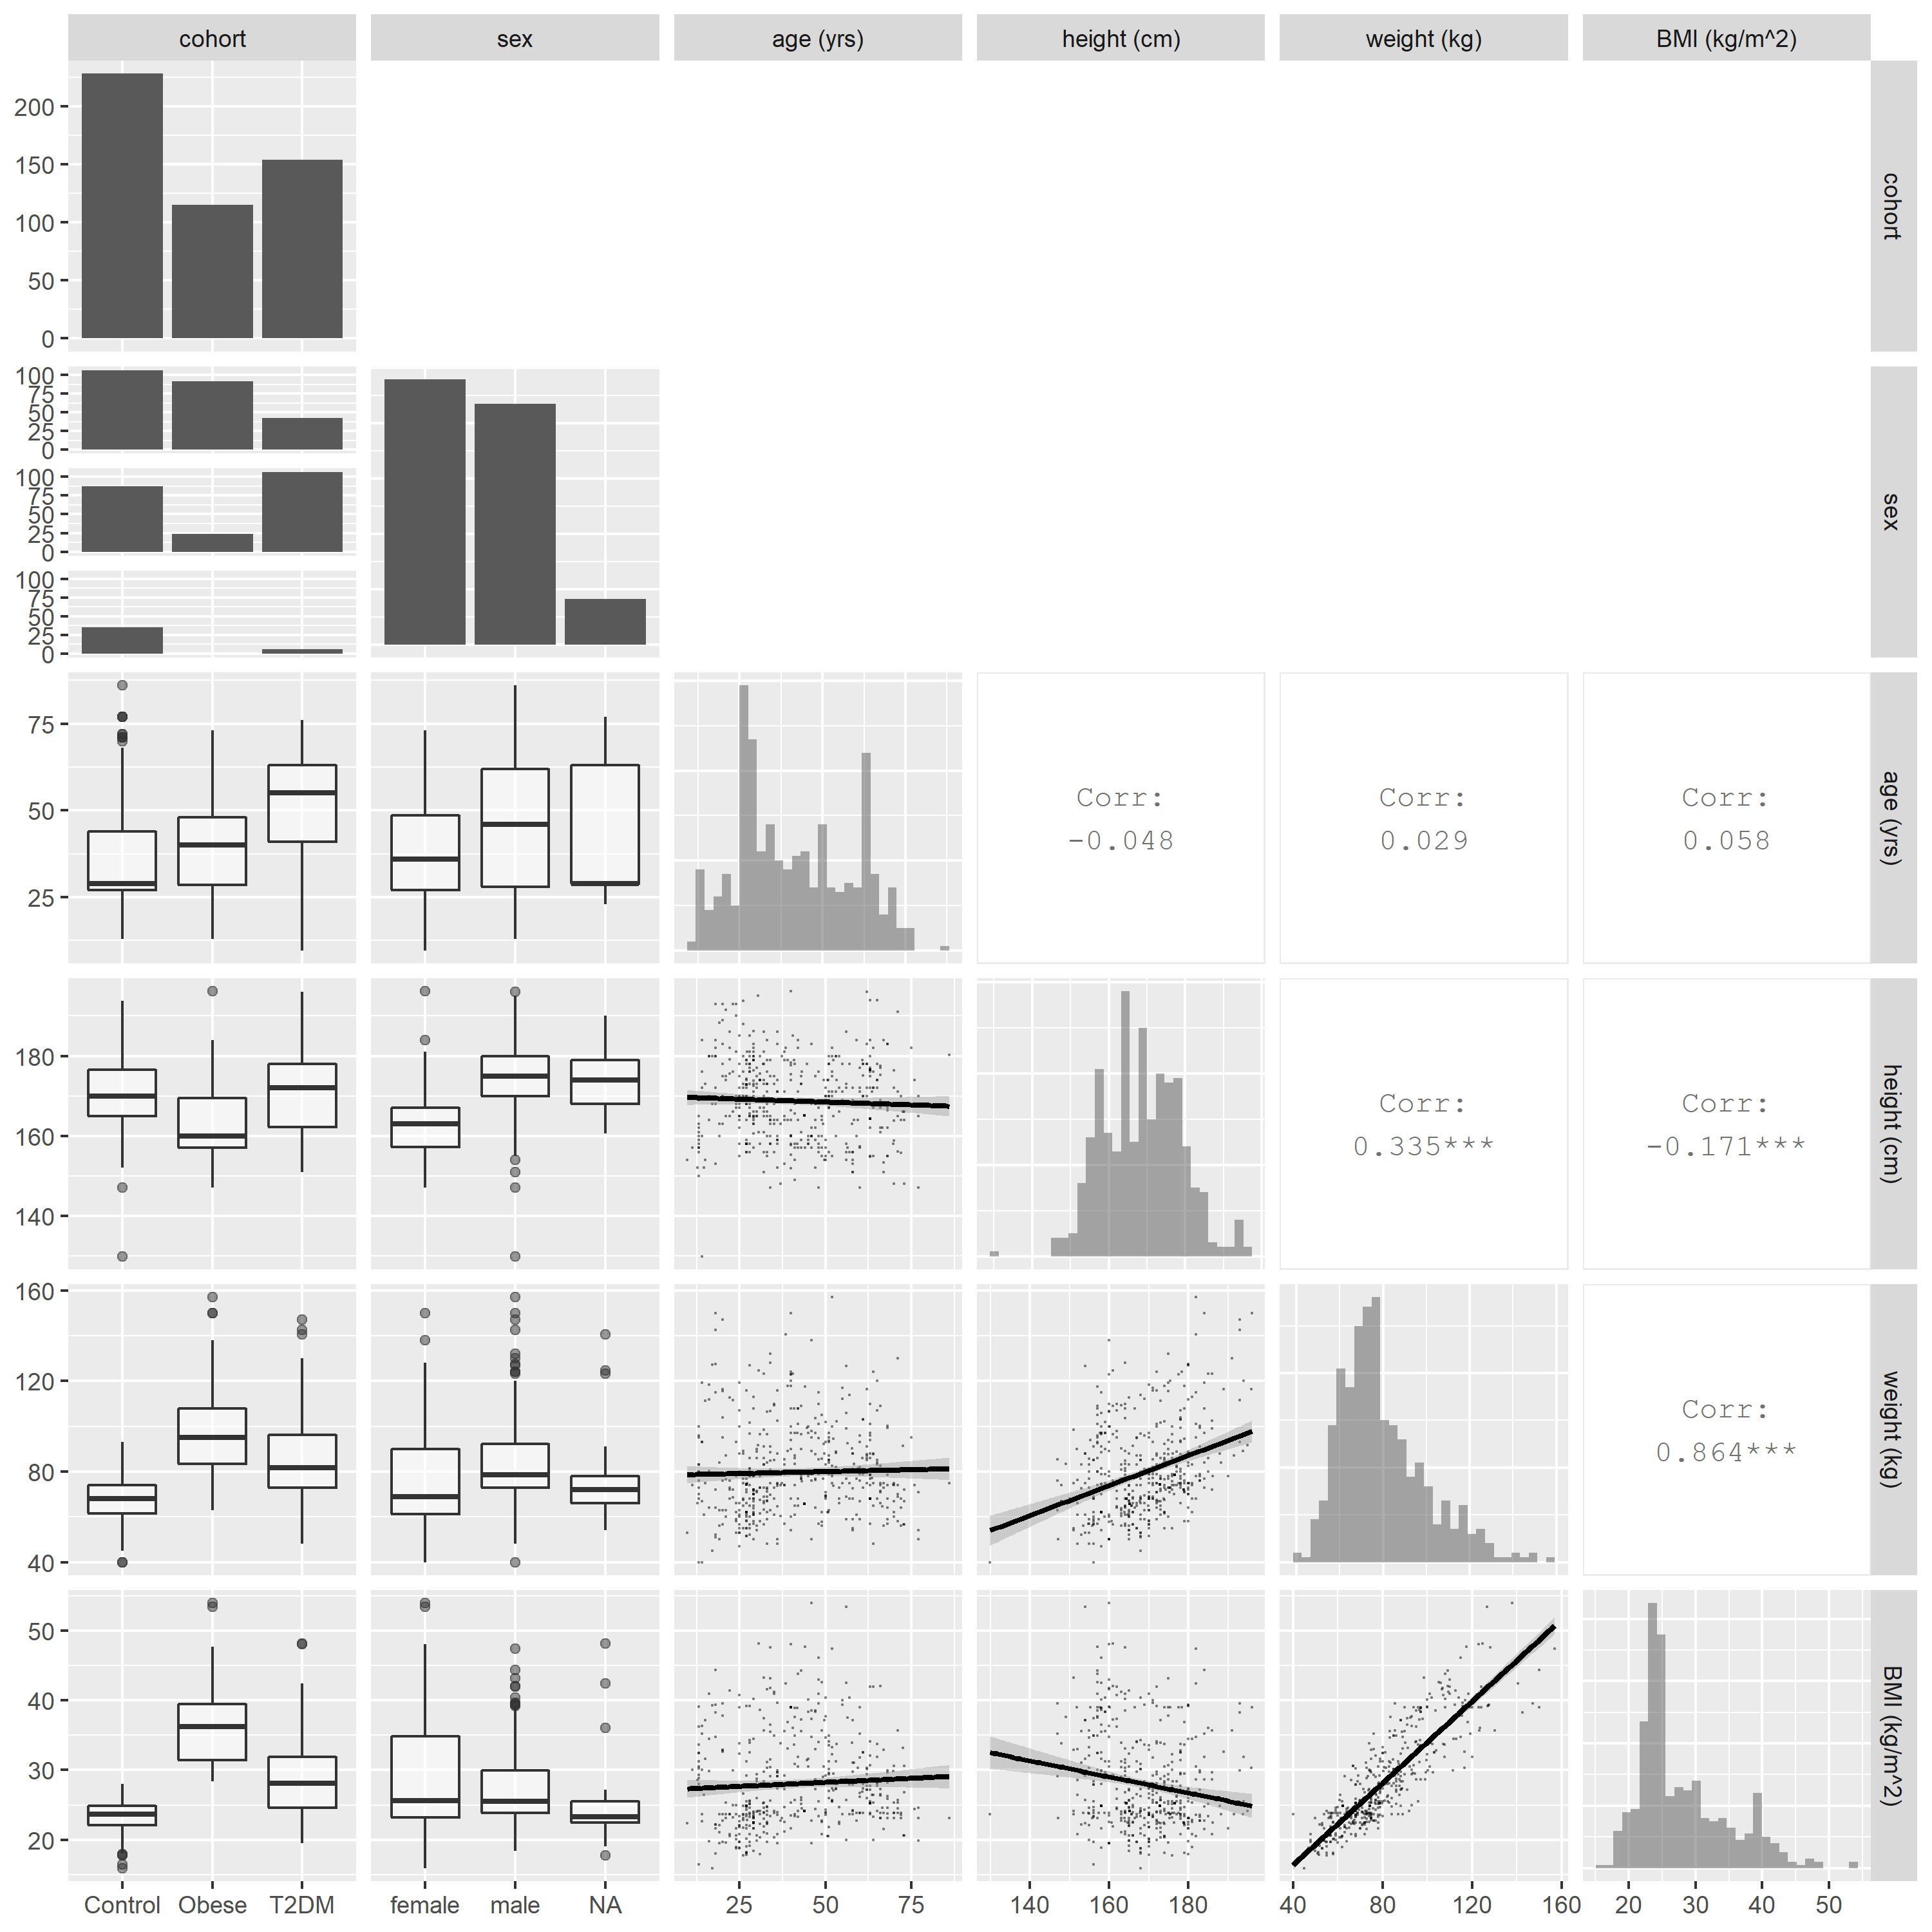
\includegraphics[width=15cm]{p2.PNG}
\end{center}
\caption{Overview of covariate values and relationships. Histograms plots for continuous covariates and bar graphs for discrete covariates are shown on the diagnoal line. In the lower triangle, the boxplots between continuous and discrete covariates and scatter plots between continuous covariates are displayed. In the upper triangle, the correlation coefficients between continuous covariates are shown.}
\label{fig: cova}
\end{figure}

\begin{figure}[h!]
\begin{center}
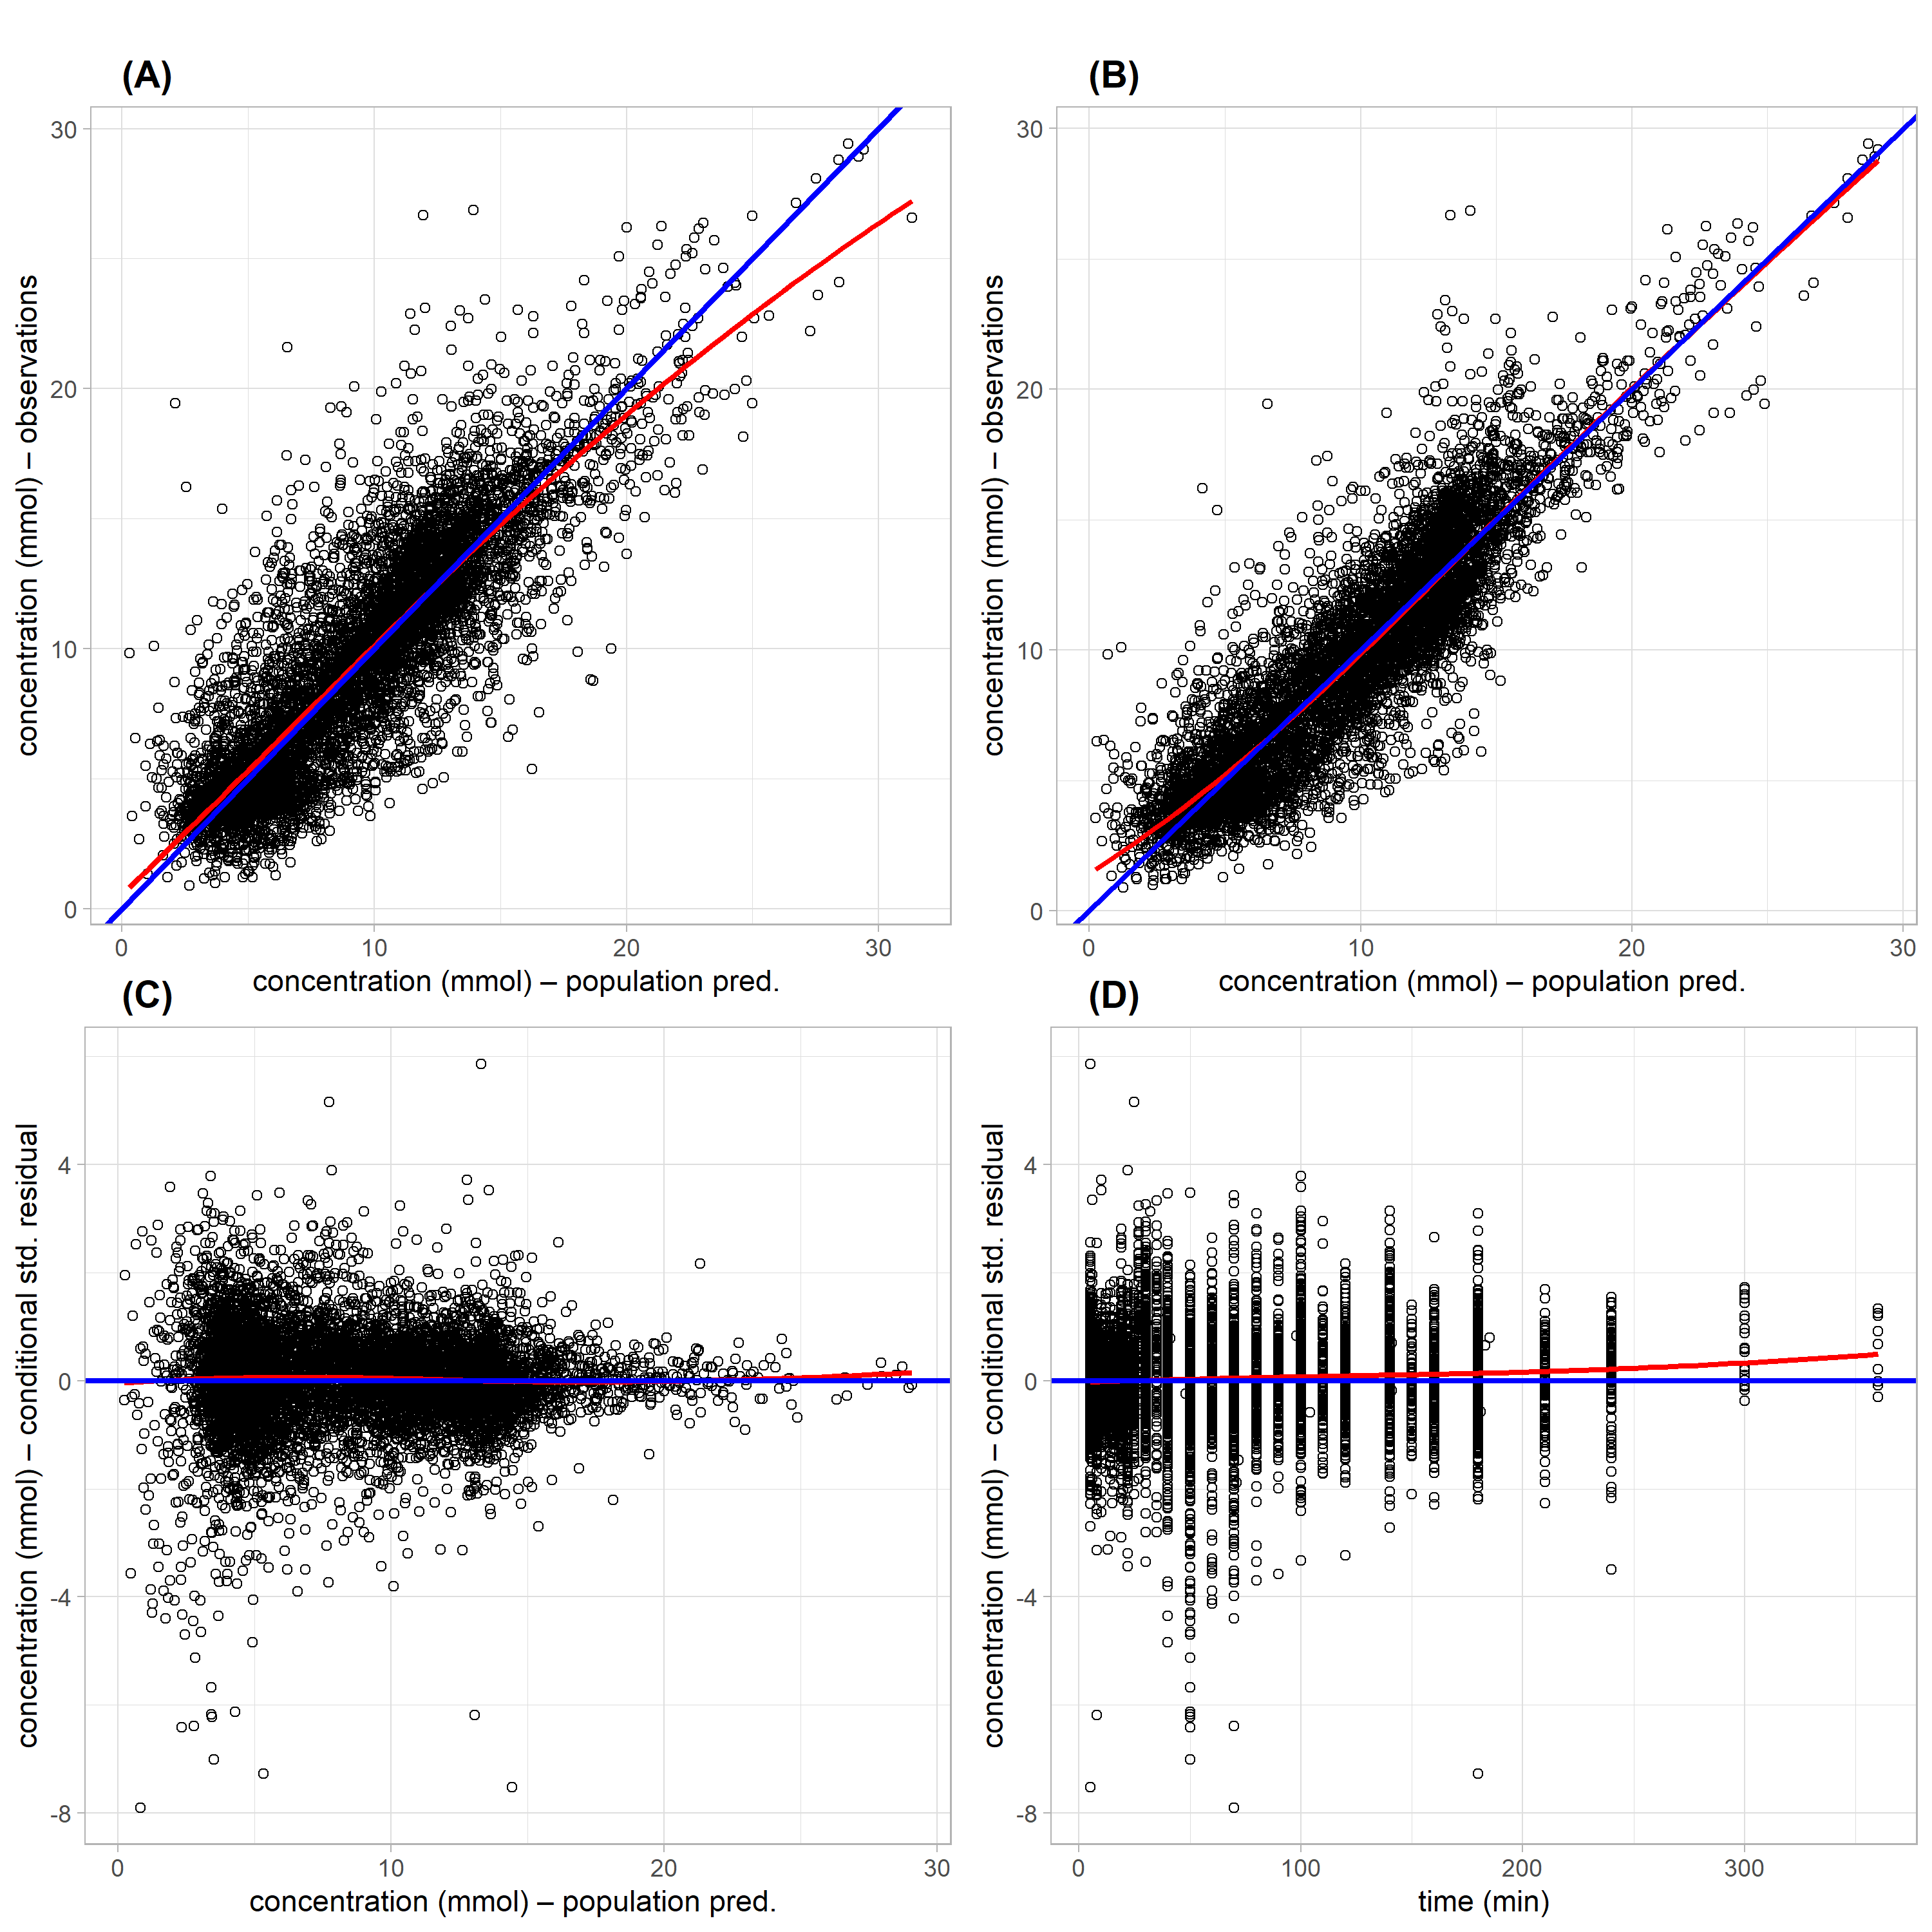
\includegraphics[width=15cm]{comb.PNG}
\end{center}
\caption{Goodness-of-fit plots}
\label{fig: fittings}
\end{figure}

\begin{figure}[h!]
\begin{center}
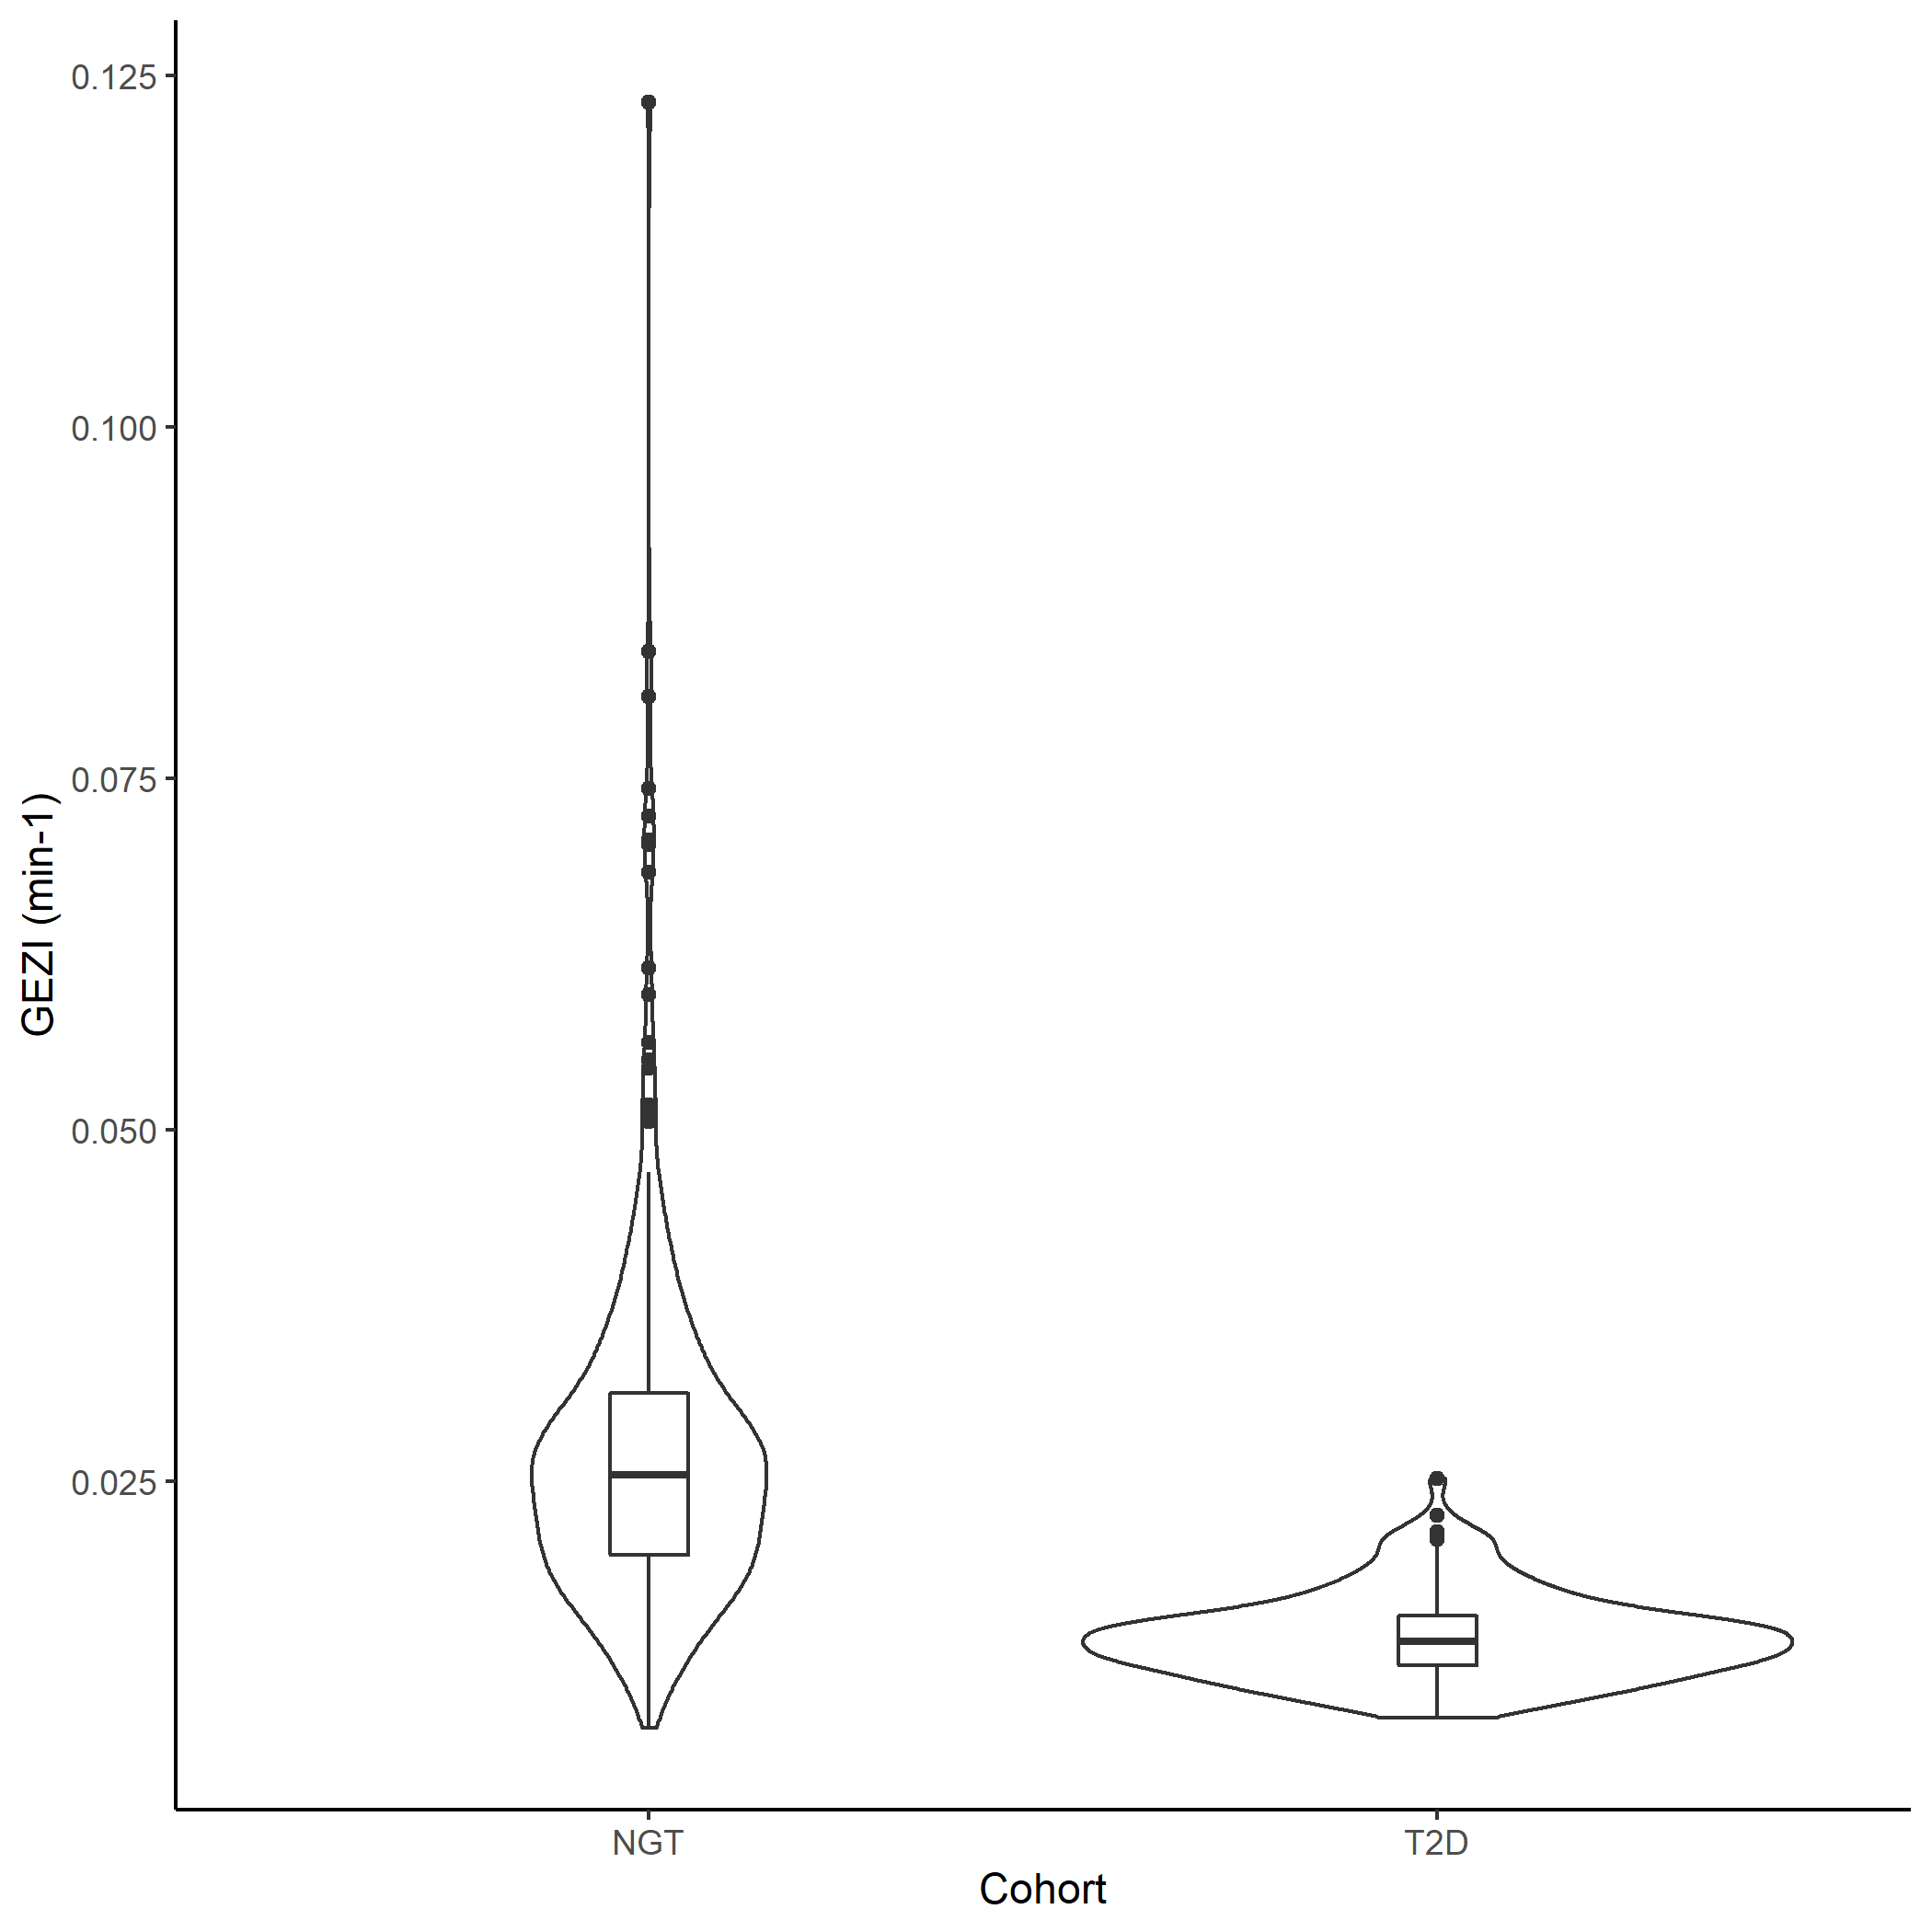
\includegraphics[width=15cm]{SG_co.PNG}
\end{center}
\caption{The distribution of $GEZI$ values by different cohorts}
\label{fig: SG_co}
\end{figure}

\begin{figure}[h!]
\begin{center}
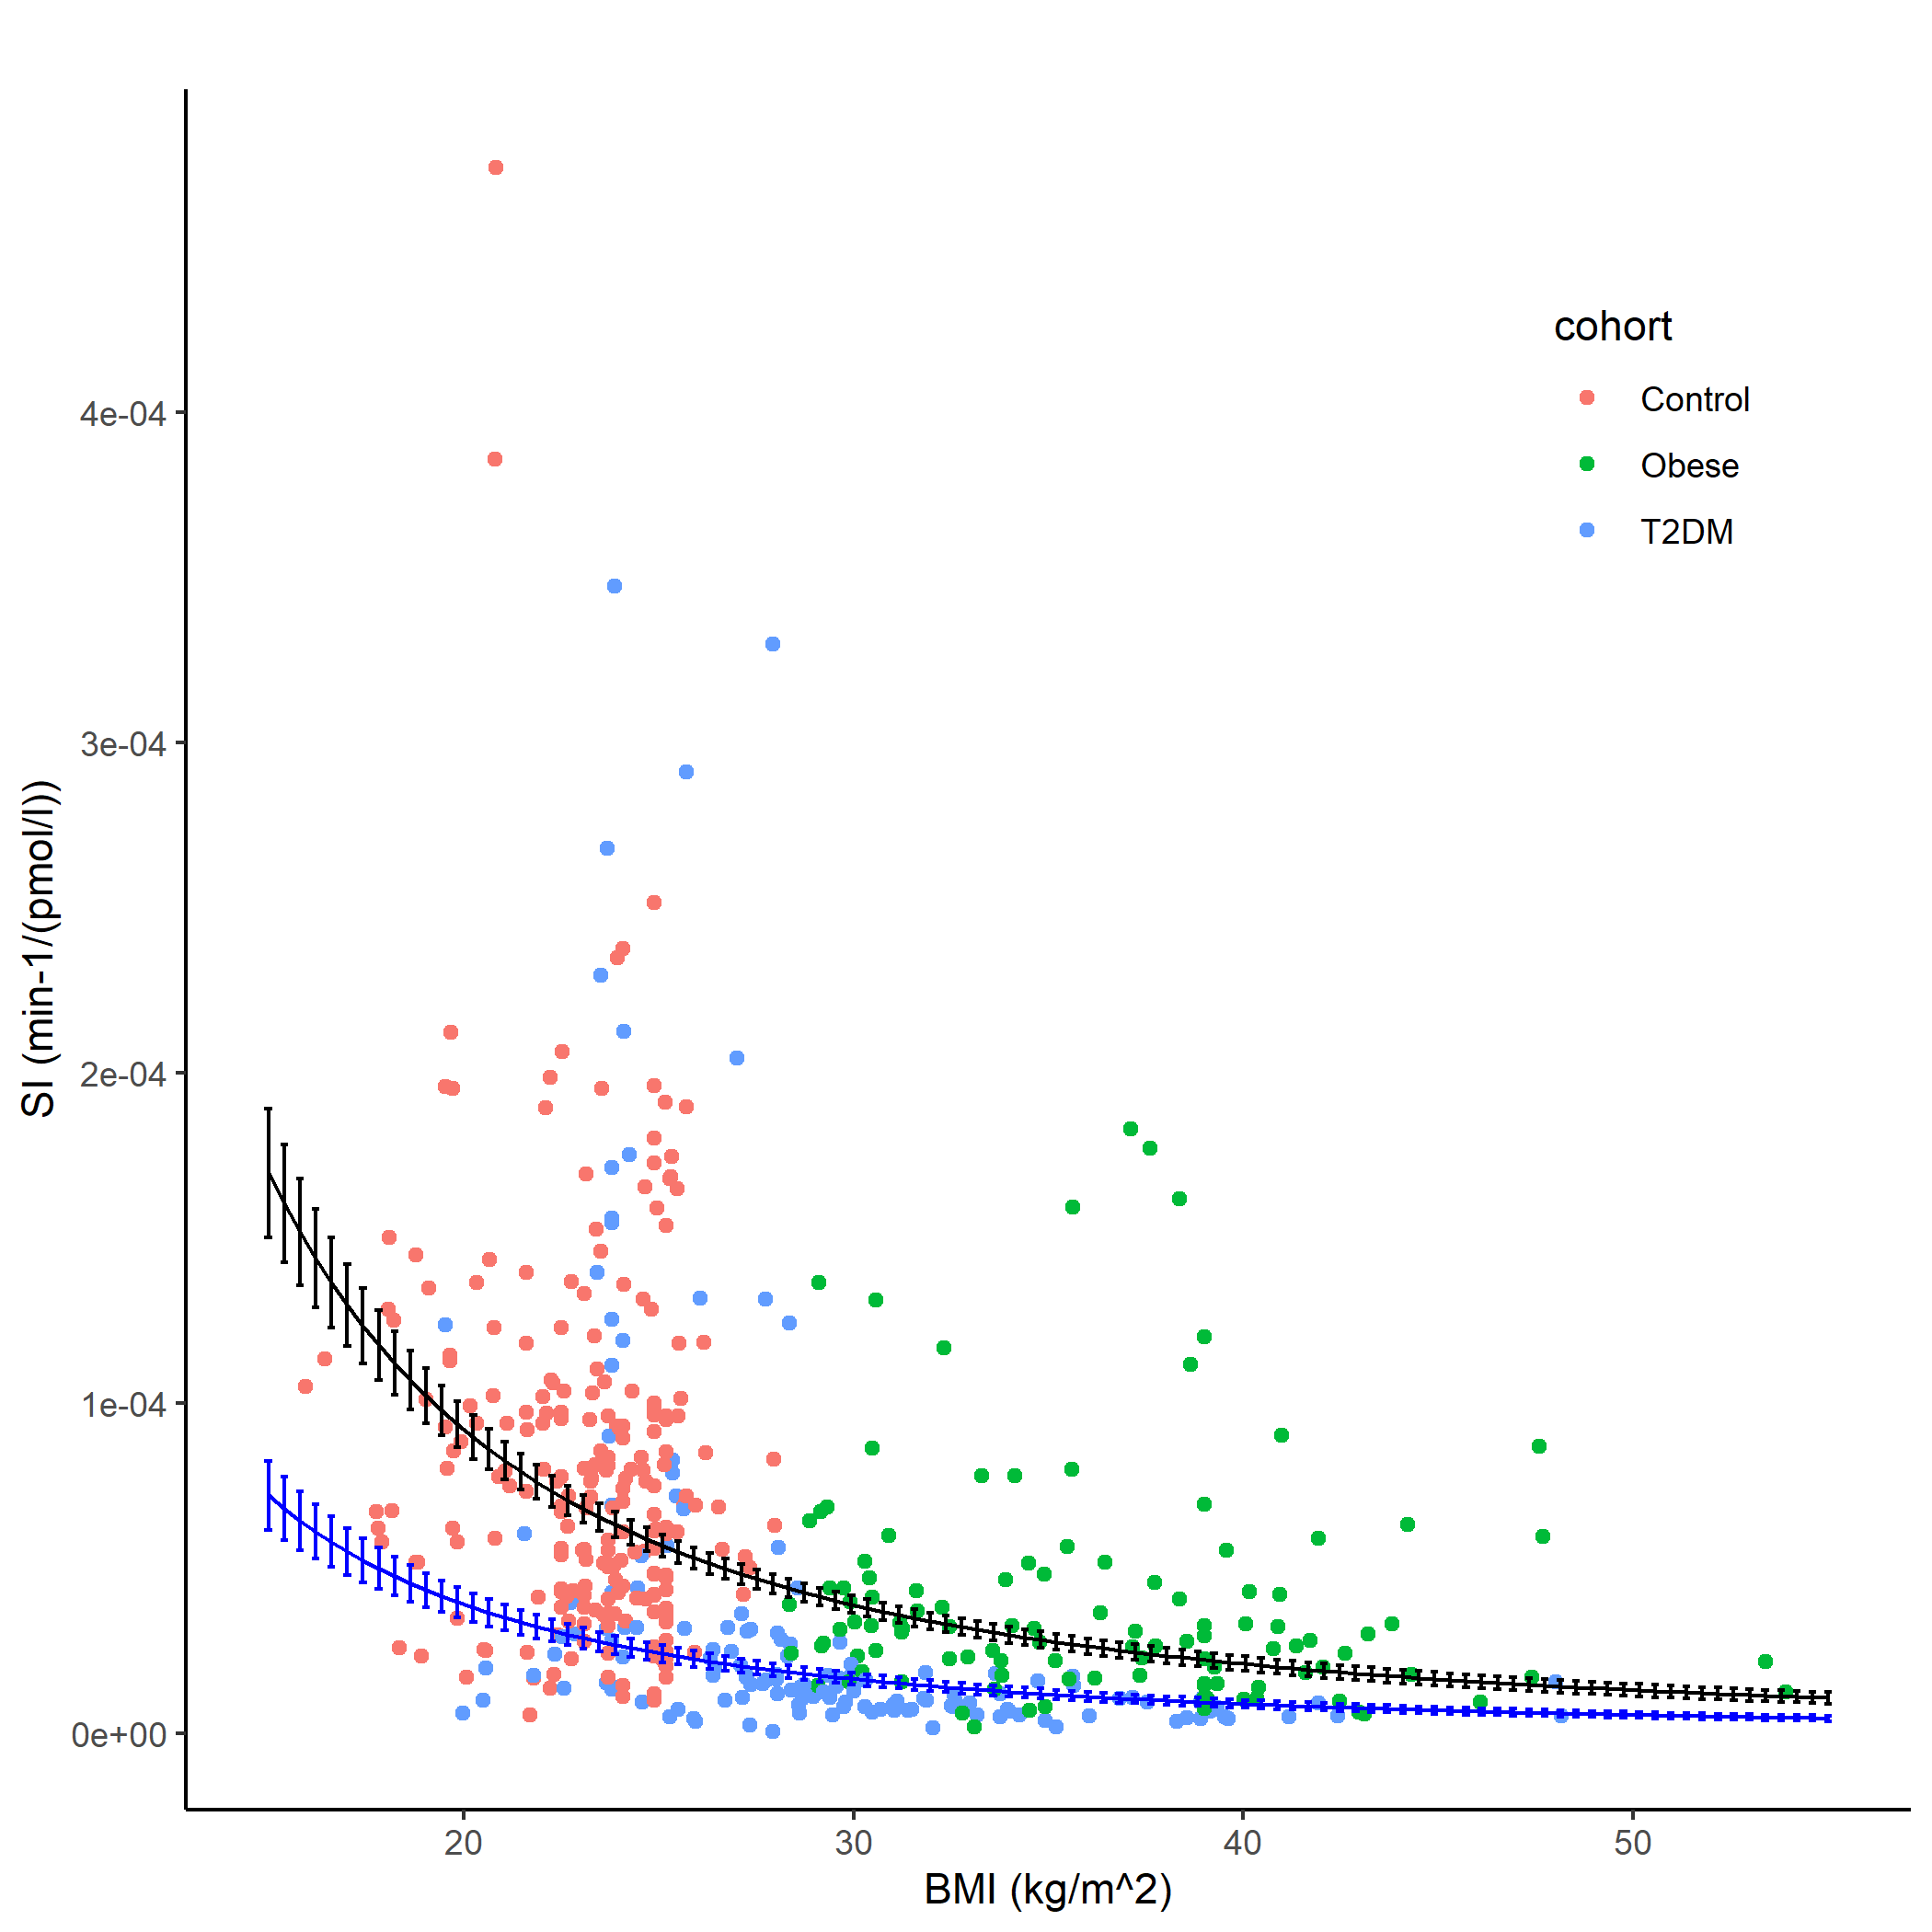
\includegraphics[width=15cm]{SI_BMI.PNG}
\end{center}
\caption{BMI effect on SI}
\label{fig: SI_BMI}
\end{figure}

\begin{figure}[h!]
\begin{center}
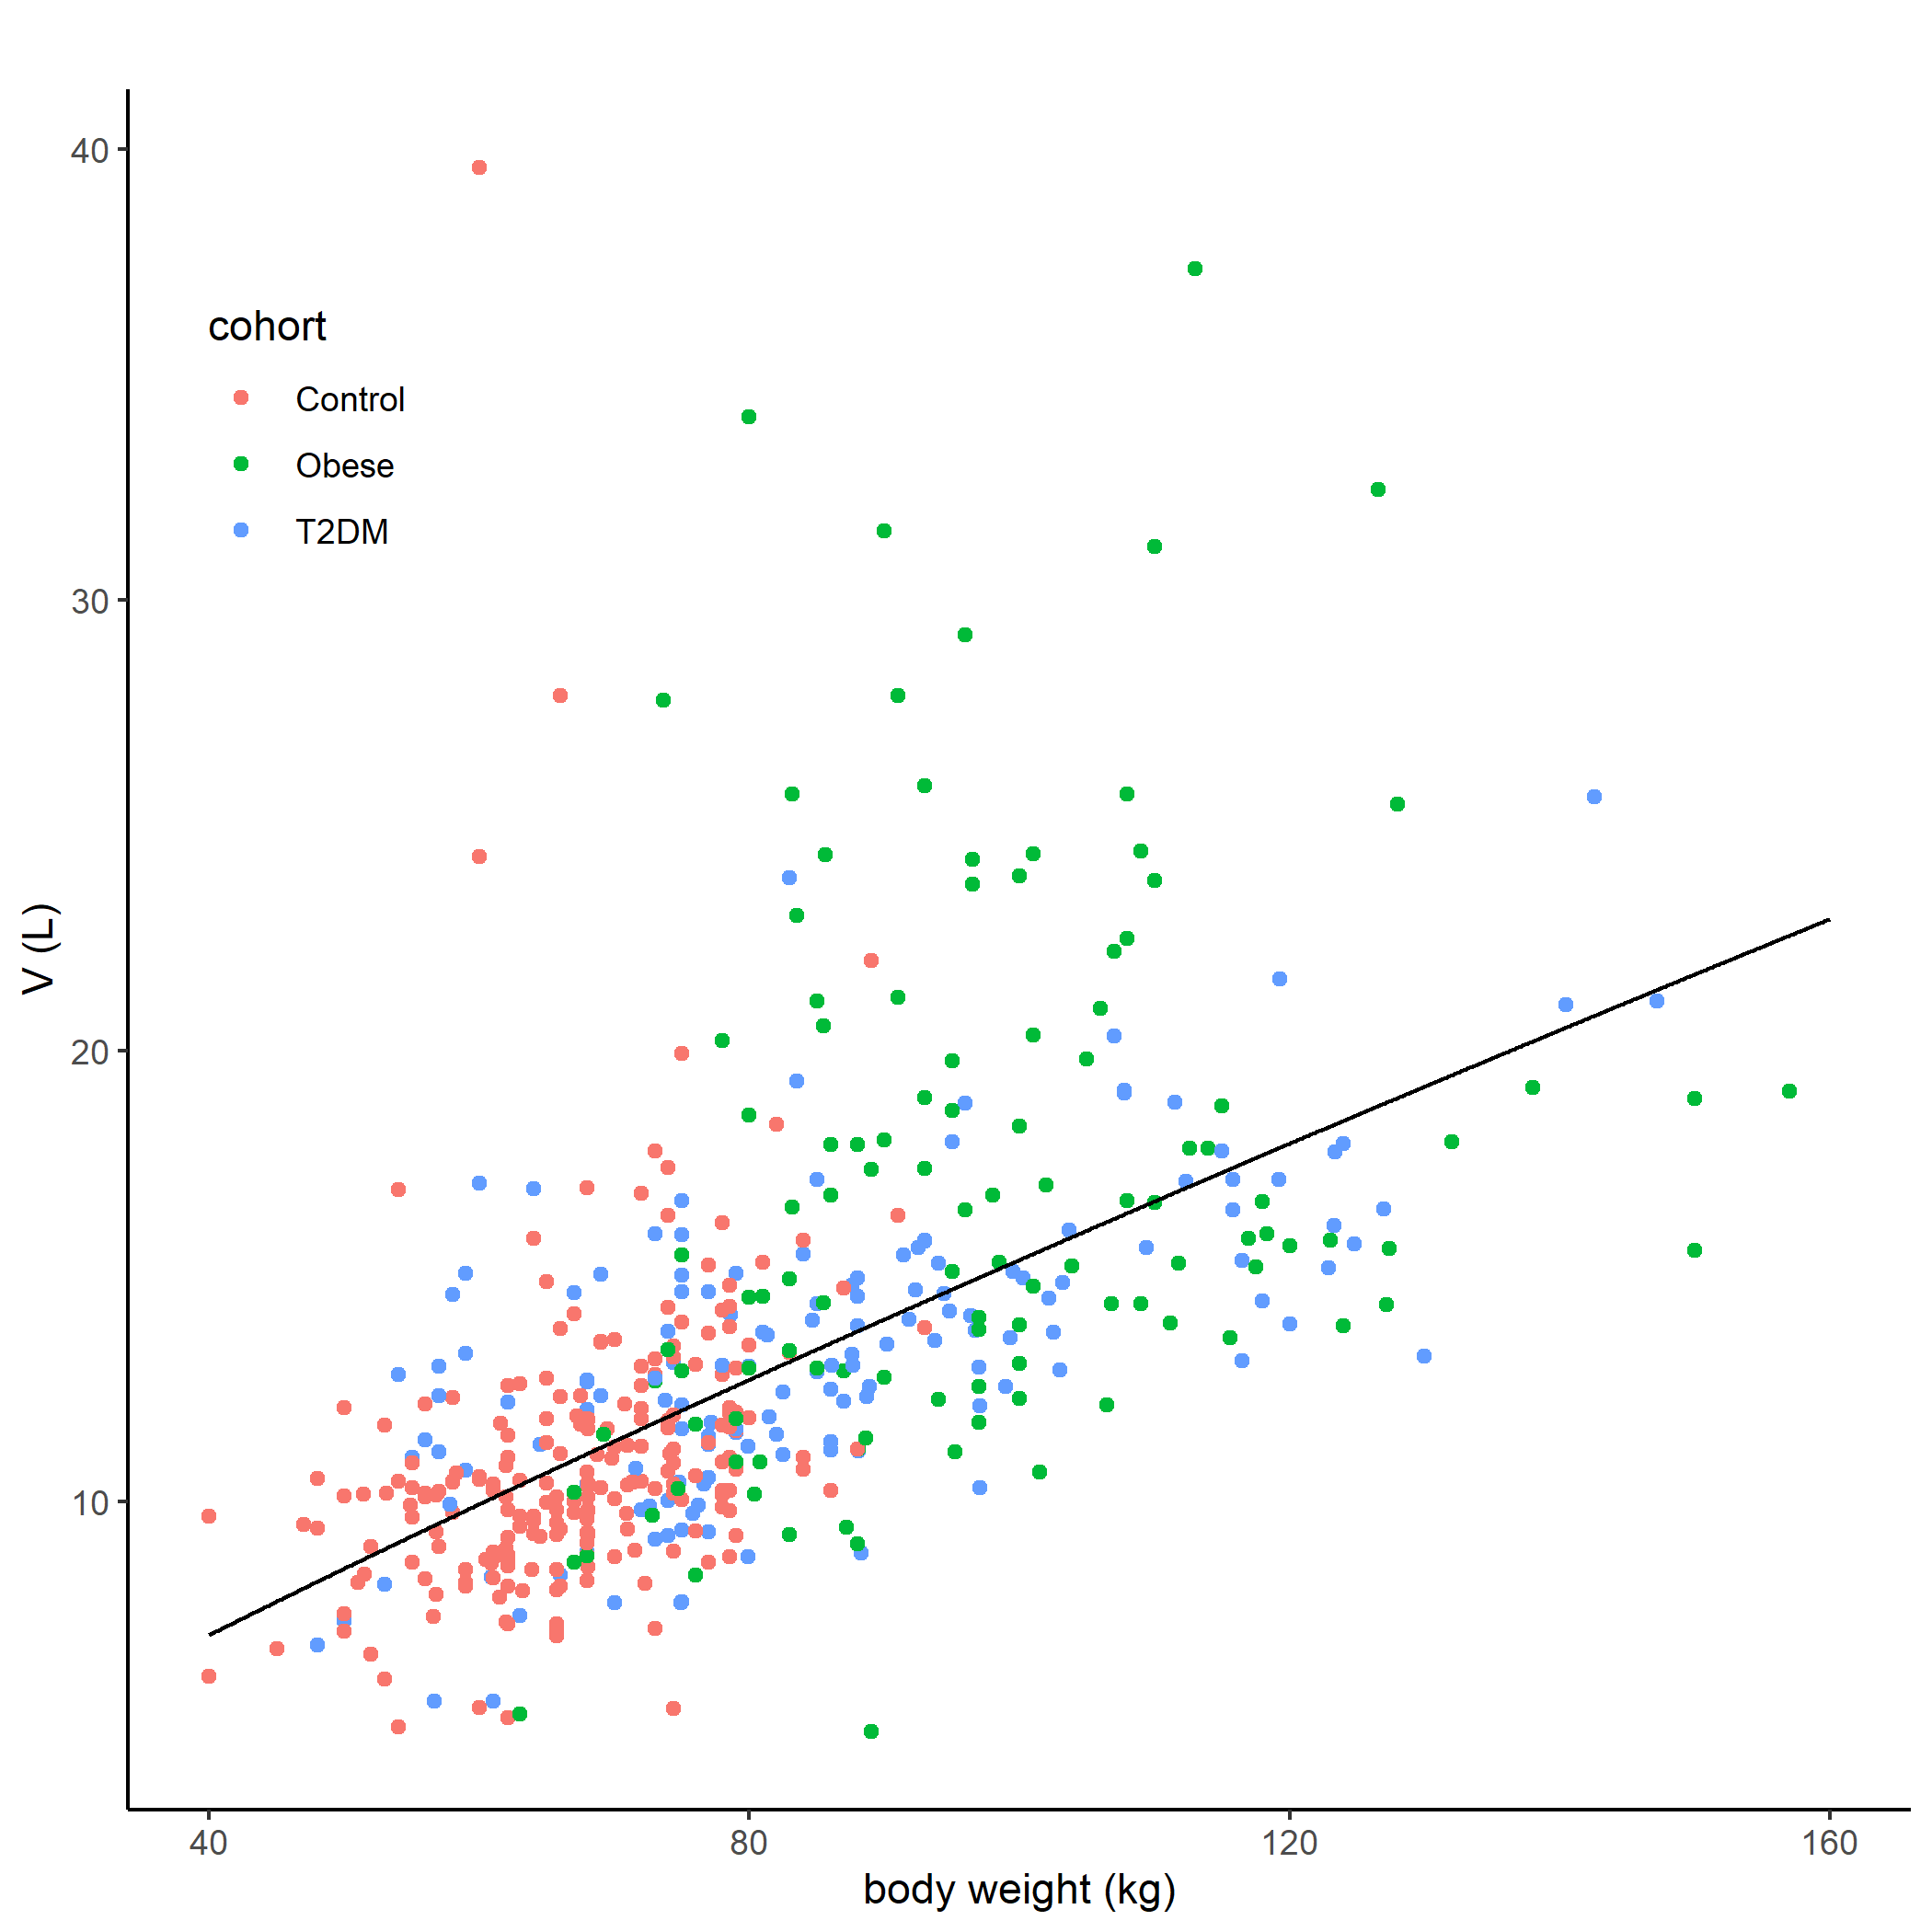
\includegraphics[width=15cm]{V_BW.PNG}
\end{center}
\caption{BW effect on V}
\label{fig: V_BW}
\end{figure}

\begin{figure}[h!]
\begin{center}
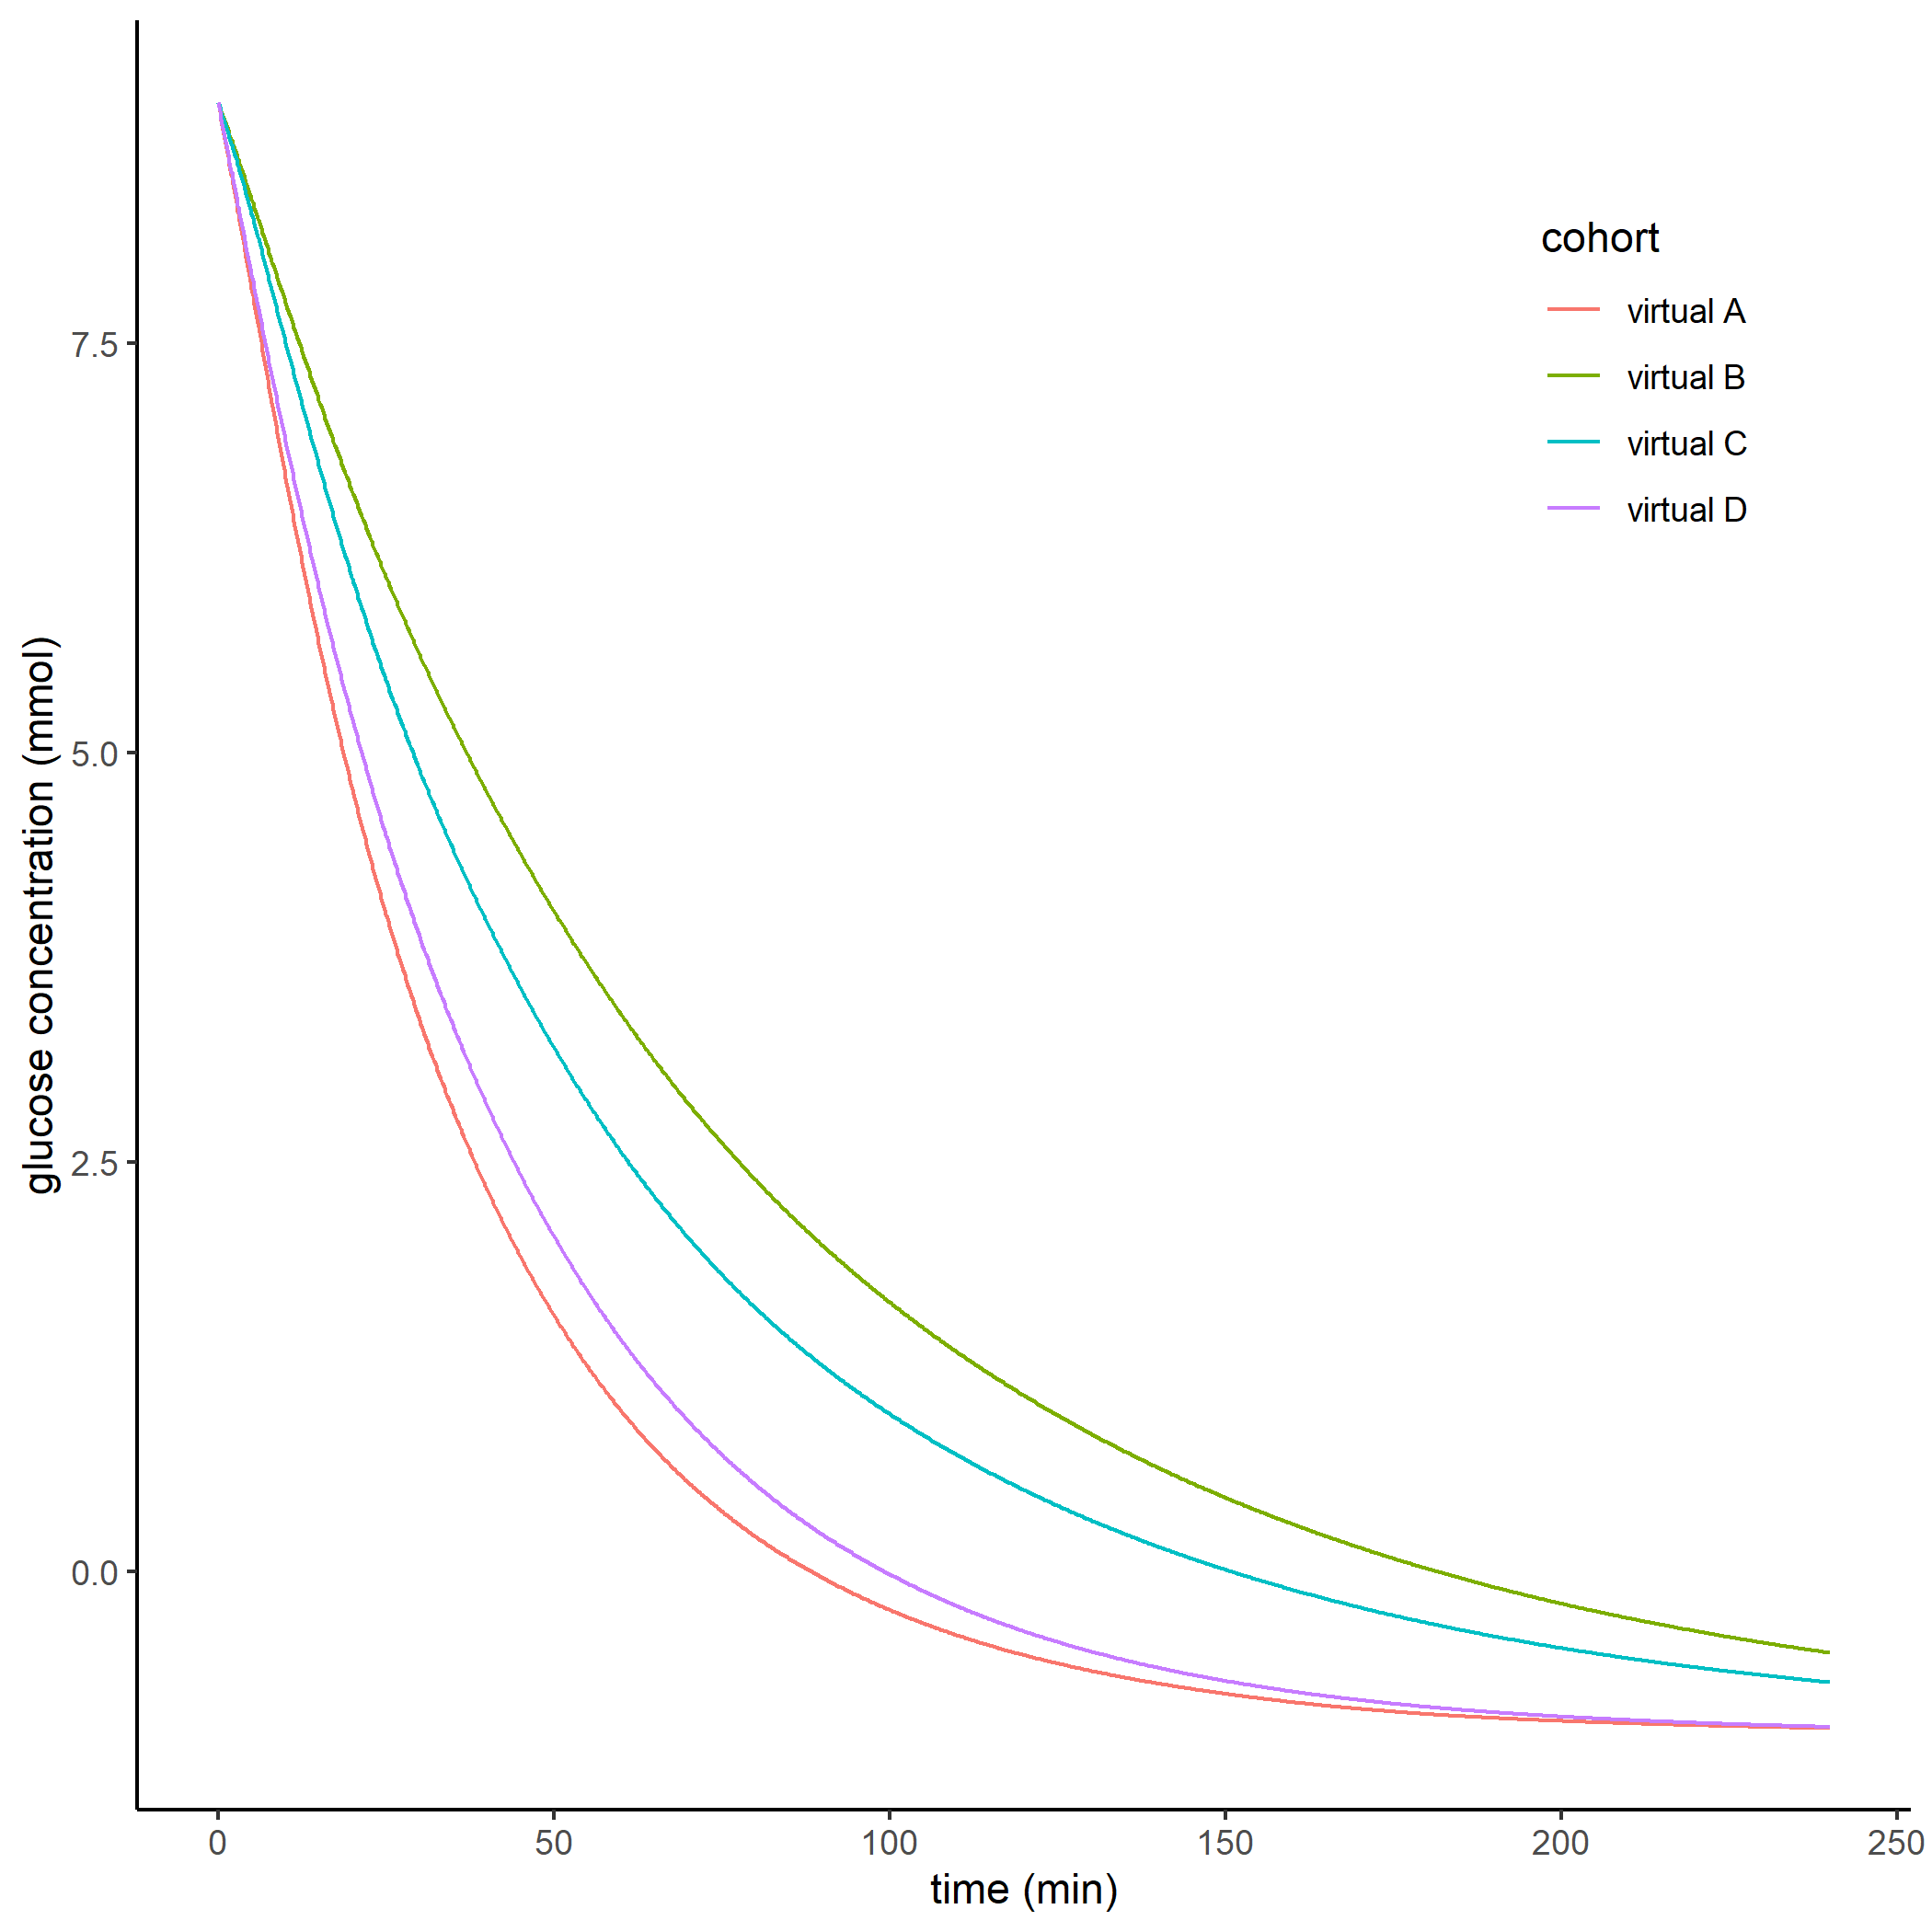
\includegraphics[width=15cm]{p.PNG}
\end{center}
\caption{Simulation of glucose concentration profile of virtual subjects with different $GEZI$ and $S_I$ values in an IVGTT. }
\label{fig: simu}
\end{figure}

\end{document}


